\section{Practicing Stage}

The practicing stage optimizes the parameters of each control rig
selected by the coaching stage. Although the search space is
largely reduced by using control rigs rather than low-level control
variables, we still need to solve a non-convex and discontinuous
optimization problem. Much previous work in computer animation applied
Covariance Matrix Adaptation Evolution Strategy (CMA-ES) to problem in
this nature. The standard procedure at each iteration involves
generating samples in the control variable space, using the samples to
simulate motions, and evaluating each motion according to the cost
function. 

However, the standard CMA-ES does not exploit two distintive
features of our problem. First, our problem has a clear
definition of infeasible samples, such as the control parameters that
result in an imbalanced motion. Second, because our framework is an
iterative process, we have a series of optimization problems sharing
very similar feasible regions. Without leveraging these features, the
standard CMA-ES spends much computation time on repeatedly evaluating
failed samples.

We designed a new algorithm, called CMA-C, based on the observation of
human's ability to \emph{learn from failure}. Because failure in the
real world is usually associated with pain or injury, humans tend to
be very effective in characterizing the cause of failure and trying to
avoid the same mistakes in the future. To this end, CMA-C
simultaneously builds a set of Support Vector Machines (SVMs) along
with the evolution of CMA. Each SVM approximates the infeasible region
of a particular type of failure. CMA-C accelerates the optimization by
preventing redundant evaluations of failed samples. Moreover, the
constructed SVMs can be reused by subsequent optimizations because
they share similar feasible regions, further speeding up the
computation significantly.

\begin{center}
\begin{landscape}
\begin{table*}[ht]
  \center
  \caption{      
    CMA-C evaluation on five problems. CMA-C improves the
    computation by four to five times. 
    $\mu$, $\lambda$, and $\sigma$ represents 
    CMA parent size, population size, and step size.
    $\hat{\vc{C}}$, $\hat{\vc{P}}$,
    $\hat{\vc{L}}$, and $\hat{\vc{S}}$ indicate the desired COM, linear
    momentum, angular momentum, and the COP.
  }
  \small
  \begin{tabular}{ | l | p{2.0cm} | p{3.0cm} | c | c | c | c | p{0.8cm} | p{1.15cm} | c | c |}
    \hline
    Problem & Objective function & Constraints ($c_1 | c_2 |$ ...) 
    & $\mu$ & $\lambda$ & $\sigma$ & Domain
    %% & \revtwo{$K_{toy}^{f}$} & \revtwo{$K_{toy}^{inf}$}
    & \shortstack{ Feasible\\region} 
    & Noise
    & \shortstack{ CMA-ES\\ (evals/total time)} 
    & \shortstack{ CMA-C \\ (evals/total time)} \\ \hline

    Toy1 &$f(x,y)=0.1 ((x - 3.9)^2 + (y - 3.9)^2)$ & $(x > 4$ $or$ $y > 4)$ $|$ $x + y < 7.5$ 
    & 4 & 8 & 5 & $[-5, 5]^2$
    %% & 0 & 0.5
    & Convex
    & Asymmetric Random
    & 663.2 / 8ms & 144.8 / 70ms \\ \hline

    Toy2 &$f(x,y)=0.1 ((x - 3.9)^2 + (y - 3.9)^2)$ & $(x > 4$ $or$ $y > 4)$ $|$ $x + y < 7.5$ 
    & 4 & 8 & 5 & $[-5, 5]^2$
    %% & 0 & 0.5
    & Convex
    & Symmetric Undulation
    & 1026.4 / 9ms & 229.6 / 116ms \\ \hline


    Toy3 &$f(x,y)=0.1 ((x - 3.1)^2 + (y - 3.6)^2)$ &
    $(x > 4$ $or$ $y > 4)$ $|$ $(x < 3$ or 
    $y < 3$ or $(x < 3.5$ and $y < 3.5))$
    & 4 & 8 & 5 & $[-5, 5]^2$
    %% & 0 & 0.5
    & Non convex
    & Symmetric Undulation
    & 1027.2 / 10ms & 205.2 / 107ms \\ \hline

    Leaning & $\| \vc{C}(\vc{q}_f) - \hat{\vc{C}} \|^2$ & 
    Fall forward $|$ Fall backward $|$ Timeout 
    & 5 & 10 & 1 & $[-1, 1]^4$
    %% & - & -
    & -
    & -
    & 126.25 / 148s & 23.75 / 32s\\ \hline

    Thrusting & $\| \vc{P}(\vc{q}_f) - \hat{\vc{P}} \|^2 + \|
    \vc{L}(\vc{q}_f) - \hat{\vc{L}} \|^2$ & 
    Fall forward $|$ Fall backward 
    $|$ Negative angular momentum
    & 5 & 10 & 1 & $[-1, 1]^3$
    %% & - & -
    & -
    & -
    & 101.25 / 15s & 77.5 / 12s \\ \hline

    Landing & $\| \vc{C}(\vc{q}_f) - \hat{\vc{C}} \|^2 + \|
    \vc{S}(\vc{q}_f) - \hat{\vc{S}} \|^2$ & 
    Fall forward $|$ Fall backward $|$ Invalid contact 
    & 5 & 10 & 1 & $[-1, 1]^4$
    %% & - & -
    & -
    & -
    & 105.0 / 210s & 22.5 / 44s \\ \hline

  \end{tabular}
  \label{tab:parkour_cmac}
\end{table*}
\end{landscape}
\end{center}


\subsection{CMA-C}
\label{sec:parkour_ccma}

CMA-C is designed for solving a general optimization problem with
multiple constraints.

\begin{equation}
  \begin{aligned}
    \vc{x}^{*} = & \argmin_{\vc{x}} f(\vc{x}) \\
    \text{subject to} & \text{ $c_i(\vc{x}) = 0$, where $i = 1 \cdots n$}
  \end{aligned}
  \label{eq:parkour_generalproblem}
\end{equation}

In our formulation, the cost function $f(\vc{x})$ evaluates the
performance of the simulated motion generated by a given set of
control rig parameters (\ie $\vc{x}$ refers to $\mathcal{P}$). Each
constraint $c_i(\vc{x})$ represents a type of failure when the motion
cannot satisfy it. $c_i(\vc{x})$ can be in the form of inequality
constraint, but we only show equality constraints for clarity. CMA-C
can be applied to any problem with the form of
\eqnref{parkour_generalproblem}, but it is particularly effective when
evaluating $f(\vc{x})$ is costly or when the problem is highly
constrained.

%% %% Soft constraints
%% \revthree{
%% Soft constraints using quadratic energy have been popular for regulating
%% the character's motion, but we found that hard contraints are more applicable
%% to our scenarios due to their binary behaviors.
%% For instance, an invalid contact of knees can be formulated as
%% a soft constraint using the squared distance to the ground.
%% However, this is not in favor of optimization because
%% knees need to be closed to the ground when the character prepares jumping.
%% }

%% first, some constraints in highly dynamic motions have binary behaviors.
%% For instance, invalid contacts of knees may be translated into a distance 
%% to the ground penalty but knees need to be closed to the ground 
%% when the character prepares jumping.
%% Second, same constraints may require different formulations for different motions.
%% For preventing falling forward, the stationary position of COM is important in
%% the standing motion, while the momentum becomes dominant in the landing.
%% Therefore, soft constraints require task specific designs and
%% hard to be generalized for all cases.
%% }
%% \sehoon{Make it clear and shorter}

%% For instance, invalid contacts of knees can be illustrated as a soft constraint,
%% such as a distance of knees to the ground. 
%% However, knees needs to be closed to the ground when the character prepares
%% jumping: as long as knees does not touch the ground, the motion is valid.

%% For example, preventing falling forward requires different penalties
%% in standing and landing motions: 


Our main idea is to construct classifiers using SVMs while running
CMA. For each constraint, we build a SVM to represent its feasible
region. Every time a sample is randomly drawn, we first use SVMs to
predict whether this sample will satisfy all constraints. If so, we
evaluate it using $f(\vc{x})$. Otherwise, the sample is discarded
without evaluation. In the context of our problem, we use SVMs to
predict whether a set of control variables yields successful motion
before we simulate it. If a sample is predicted to satisfy all the
constraints, we evaluate its cost and assign a label for each SVM:
$+1$ if the sample indeed satisfies the corresponding constraint and
$-1$ otherwise. At the end of each CMA iteration, we refine the
boundary of each SVM using all the samples. Algorithm \ref{alg:ccma}
and \ref{alg:selection} outline the procedure of CMA-C.

\begin{algorithm}
  %% \SetAlgoLined
  %% \KwData{this text}
  %% \KwResult{how to write algorithm with \LaTeX2e }
  Initialize $\vc{m}, \mat{C}, \sigma$\;
  Initialize $SVM_{1..n}$\;
  \While{not terminate}{
    \For{$i = 1 \to \lambda$} {
      $\vc{x}_i$ = selectSample($\vc{m}, \mat{C}, \sigma, SVM_{1..n}$)\;
      $(f_i, e_{i,1}, ... , e_{i,n})$ = fitness$(\vc{x}_i)$\;
    }
    sort($\vc{x}_{1..\lambda}$)\;
    ($\vc{m}, \mat{C}, \sigma$) = updateCMA($\vc{x}_{1..\lambda}, f_{1..\lambda}, \vc{m}, \mat{C}, \sigma$)\;


    \For{$i = 1 \to n$} {
      \If{enough samples for $SVM_i$ and $\gamma_i$ is null} {$\gamma_i = 1/2(k\sigma)^2$}
      updateSVM($SVM_i, \gamma_i, \vc{x}_{1..\lambda}, e_{1..\lambda, i}$)\;
    }
  }

  \caption{CMA-C}
  \label{alg:parkour_ccma}
\end{algorithm}
\begin{algorithm}
  %% \SetAlgoLined
  \KwData{$\vc{m}, \mat{C}, \sigma, SVM_{1..n}$}
  \KwResult{  selected sample $\vc{x}$}

  \While{  not reach maximum trials }{
    $\vc{x}$ = gaussianSelection$(\vc{m}, \sigma^2\mat{C})$\;
    $reject = False$\;
    \For{$i = 1 \to n$} {
      \If{$SVM_i$.activated() and $SVM_i$.predict($\vc{x}$) $< 0$} {
        $reject = True$\;
        break\;
      }
    }
    \If{not reject} {
        \Return $\vc{x}$
    }

  }
  \Return gaussianSelection$(\vc{m}, \sigma^2\mat{C})$\;
  \caption{selectSample()}
  \label{alg:parkour_selection}
\end{algorithm}


When the SVM makes a correct prediction,  it speeds up the convergence
of CMA. When the SVM makes an incorrect prediction (\ie generates a
sample with $-1$ label), our algorithm
still utilizes the negative sample to improve the boundary of the feasible
region. However, there are two
%% \karen{two}
%% \updated{three}
issues with this algorithm when applied in practice. 
%% First, SVMs are very inaccurate at the beginning of the optimization due 
%% to the lack of samples. 
%% Second, although SVMs can use kernels to represent non-linear boundaries, tweaking
%% kernel parameters in SVMs can greatly affect the results of classification.
%% \updated{Third, SVMs will be activated only when the distribution of the samples
%% reaches the boundary of the SVMs and have less chance to affect the optimization}
First, a SVM requires a sufficient number of positive and
negative samples before it can be activated. This requirement
imposes a long ``warm-up'' time if the initial CMA distribution has
low likelihood to generate feasible samples. 
Second, although SVMs
can use kernels to represent non-linear boundaries, tweaking kernel
parameters in SVMs can greatly affect the results of
classification.


The first issue is exasperated by problems with a large number
of constraints and a relatively small feasible region, such as the
problem of developing parkour controllers. To reduce the warm-up
time, we represent each constraint with a SVM individually, instead
of using one aggregate SVM to represent the intersection of all
constraints. During the optimization, we superimpose all the
activated SVMs and approximate the feasible region by taking the
intersection of all positive regions. Building multiple SVMs
significantly reduces the warm-up time because a positive
sample for an aggregate SVM must satisfy all constraints, where as a
positive sample for each separate SVM only needs to satisfy one
constraint. Collecting enough positive samples to activate an
aggregate SVM clearly takes much longer time than activating each
individual SVM (Figure \ref{fig:parkour_cmacwork}).  
In our toy problems, the first SVM is constructed after 17.2 evaluation
on average, an aggregate SVM requires 101.7 evaluations. 

In addition, we propose a stochastic sampling scheme to address
the general issue due to insufficient samples at the beginning of
the optimization. This scheme accepts a sample with the probability
of a sigmoid function $\frac{1}{1+e^{-\alpha x}}$, where $x$ is the
signed distance from the sample to the boundary. With a smaller
$\alpha$, this stochastic scheme is more conservative about
accepting and rejecting samples. As more samples are available and
the SVM boundary becomes more accurate, we can increase $\alpha$ to
have a harder rule. In our experiments, we use $\alpha = 4$
throughout the entire optimization.

The second issue regards the tuning of the kernel parameters. We chose
a frequently used kernel, Gaussian radial basis function (RBF), in our
implementation.
\begin{equation}
  k(\vc{x}_i, \vc{x}_j) = exp(-\gamma\|\vc{x}_i - \vc{x}_j\|^2)
\end{equation}
Intuitively, a RBF adds a ``bump'' around each sample. The bump with
the ideal size, determined by $\gamma$, should overlap with a few
neighboring samples.  If $\gamma$ is too large, the trained SVMs will
over-fit the data. If it is too small, the classification will have
very low accuracy. Consequently, tuning $\gamma$ requires the
knowledge of the current sample distribution.

Fortunately, we know the exact sample distribution because all the
samples are drawn from the current estimate of Gaussian distribution,
$\vc{x}$ \mytilde $N(\vc{m}, \sigma^2\mat{C})$, provided by CMA. With
this information, we set $\gamma$ to cover only portion of the current
CMA gaussian distribution, using a simple rule:

\begin{equation}
  \gamma = 1/2(k\sigma)^2
\end{equation}
where $k$ determines the proportion of the radial basis
function with respect to the sample distribution. We use
$k = 0.1$ for all the experiments.

\begin{figure}[tb]
  \center
  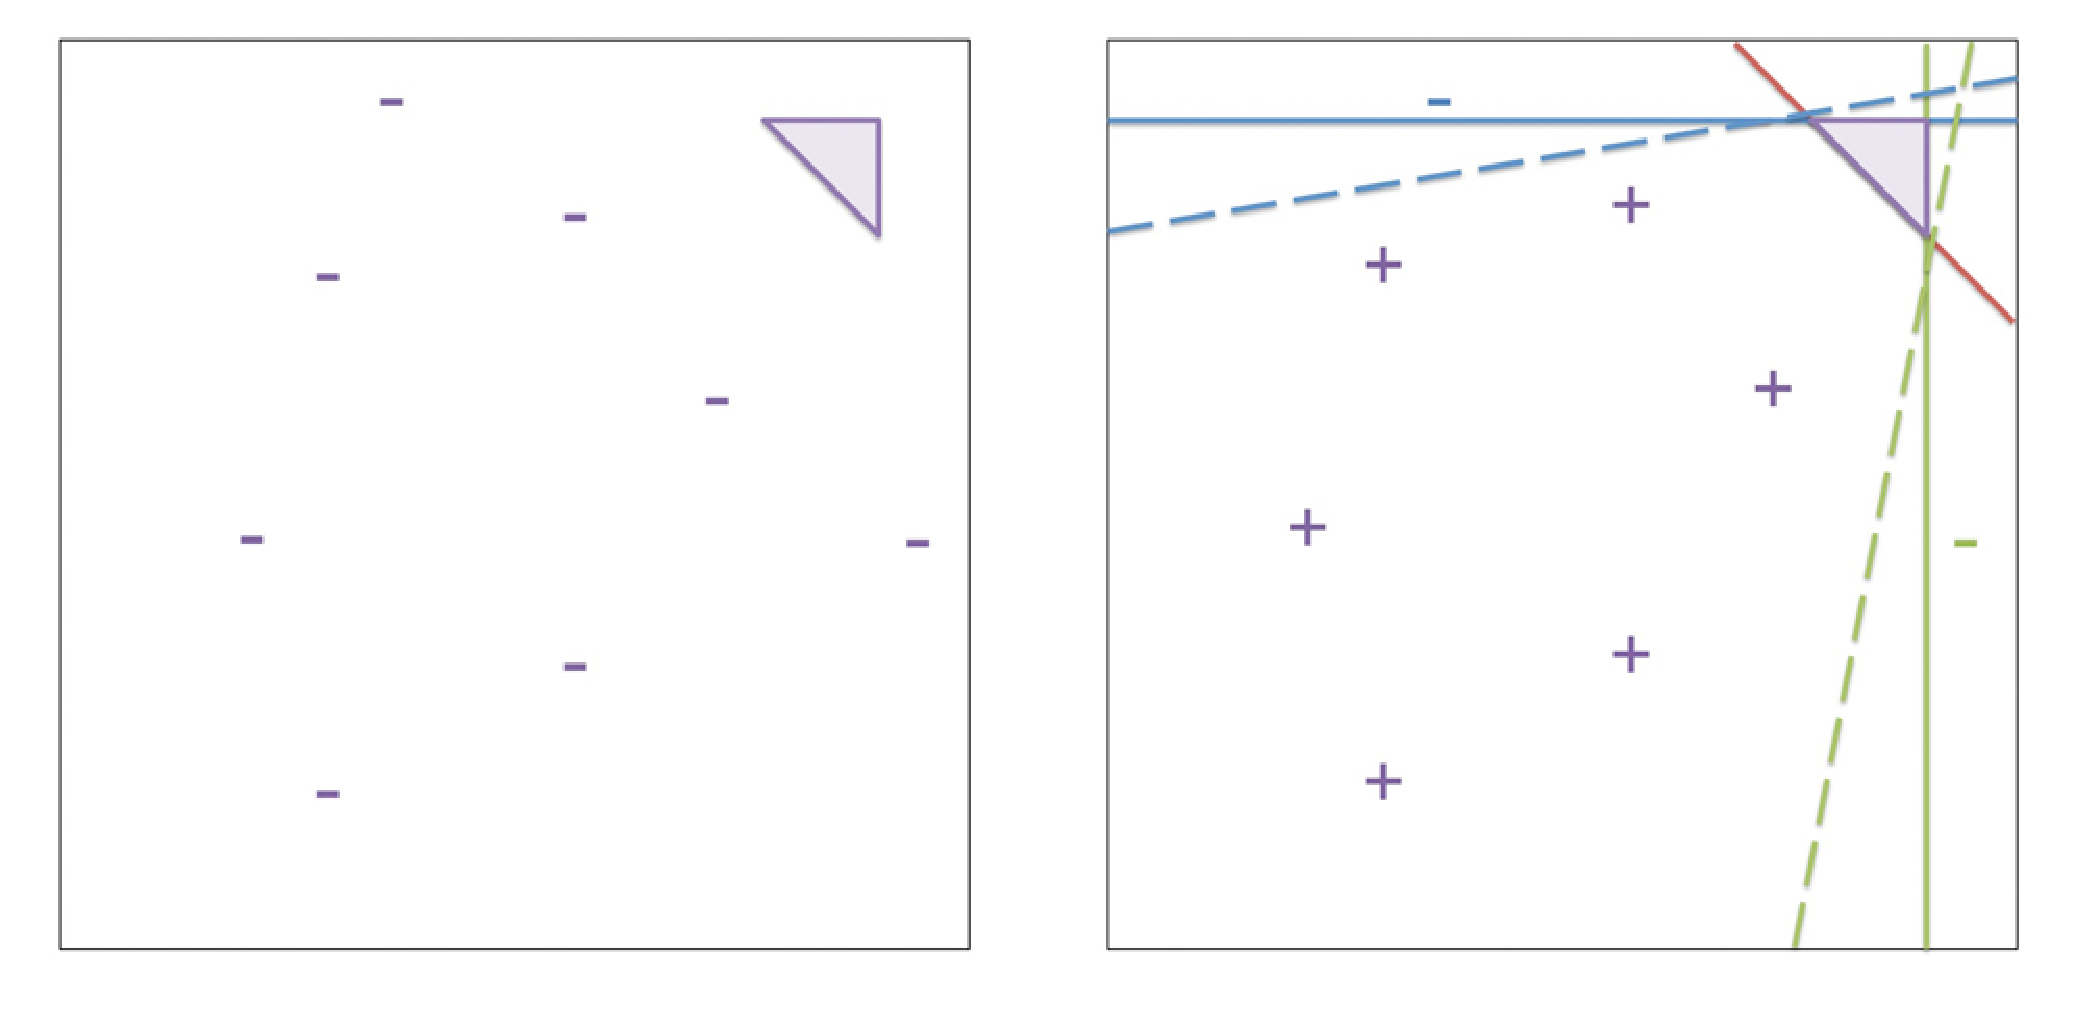
\includegraphics[width=0.75\linewidth]{images/cmacwork2}
  \caption{
    A comparison of a single SVM and multiple SVMs. Left:
    Using a single SVM to represent the feasible region (purple
    triangle), the SVM cannot be activated after eight samples, due
    to the lack of positive samples. Right: If the feasible regions
    is represented by the intersection of three constraints, each of
    which is approximated by an individual SVM, eight samples are
    sufficient to active two SVMs (shown
    in green and blue). Dashed lines indicate the current SVM
    approximation of constraints.
  }
  \label{fig:parkour_cmacwork}
\end{figure}


%% \updated{ The last issue happens because SVMs cannot accelerate the
%%   optimization when CMA searches the complete inside or outside of
%%   SVMs.  If the problem is difficult, it is very likely to waste a lot
%%   of time before activating SVMs.  Our key intuition is finding a
%%   feasible region for each constraint is much easier than finding a
%%   grand solution which satisfies all the constaints.  For instance, a
%%   challenging task of stable landing becomes easier if we focus on
%%   making the right contact with feet (Invalid contact constraints) at
%%   first, and then work on balancing problem (Fall forward/backward
%%   constraints).  Therefore, superimposing of multiple SVMs is an
%%   effective strategy to get full benefit of constructing constraints
%%   (\figref{parkour_cmacwork}).  In our toy problems with multipel SVMs, the
%%   first SVM is activated after 17.2 evaluation in average, while using
%%   a monolithic SVM takes 101.7 evaluations.  } 



\subsection{Analysis on Toy Problems}
\label{sec:parkour_toyproblems}
In addition to the real problems on motion control, we
designed three 2D problems to evaluate and visualize the results of
CMA-C. We found that CMA-C outperforms CMA-ES significantly when the
problem has a large portion of infeasible region or when the
infeasible region is highly nonlinear or discontinuous. In other
words, if the optimizer is more likely to be ``trapped'' in the
infeasible region, CMA-C has a better chance to ``escape'' and
converge at a feasible and optimal solution.

The first two toy problems have convex feasible regions, 
  while the third one has a non-convex feasible region (Figure \ref{fig:parkour_cmac}, 
  Table \ref{tab:parkour_cmac}).
To mimic the nonlinearity and discontinuity in the
objective function of the real problems, we added random noise to
the objective function of the toy problems.
For the first toy problem, we add different levels of random noise
  in feasible and infeasible regions as follows:

\begin{equation}
  \begin{aligned}
    f_{toy}(x,y) = 
    \begin{cases}
      f(x,y) + k_{toy}^{f} \cdot ( rand(0, 1) ) &  \text{ if } \forall i, c_i = 0  \\
      f(x,y) + k_{toy}^{inf} \cdot ( rand(0, 1) ) & \text{ otherwise }
    \end{cases}
    \label{eq:parkour_toyerrorfunc}
  \end{aligned}
\end{equation}

where $k_{toy}^{f}=0.05$ and $k_{toy}^{inf}=2.0$.
In the second and third problems, we add same sinusoidal noise 
in both feasible and infeasible regions:

\begin{equation}
  \begin{aligned}
    f_{toy}(x,y) &= f(x,y) \\
    &+ k_{toy} \cdot | sin(\omega_{toy}\cdot(x + y)) + sin(\omega_{toy}\cdot(x - y))|
    \label{eq:parkour_toyerrorfunc2}
  \end{aligned}
\end{equation}

where the magnitude and frequency of the
sinusoidal function $k_{toy}=2.0$ and $\omega_{toy} = 10.0$.
%% \karen{do we need to show this since we are varying these values in
%%   the experiements.}

    %% f(\vc{x}) = f(\vc{x}) + K_{toy}^{f} ( rand(0, 1) ) \text{ if } 
    %% c_i = 0 \\
    %% f(\vc{x}) = f(\vc{x}) + K_{toy}^{inf} ( rand(0, 1) ) \text{ otherwise }

\begin{table}[ht]
  \caption{CMA-C on the toy problem I (Table \ref{tab:parkour_cmac}) with various ratios of the infeasible area to the feasible area.
    All other conditions are the same.}
  \center
  \begin{tabular}{ | p{2.5cm} | p{2.5cm} | p{2.5cm} | p{2.5cm} |}
    \hline
    Area Ratio & CMA-ES (evals) & CMA-C (evals) & Performance gain \\ \hline
    50 &  237.2 & 153.2 & 155\% \\ \hline
    200 &  663.2 & 144.8 & 458\% \\ \hline
    800 & 1343.6 & 200.0 & 672\% \\ \hline
  \end{tabular}
  \label{tab:parkour_toy_area_ratio_test}
\end{table}



\begin{table}[ht]
  \caption{CMA-C on the toy problem II (Table \ref{tab:parkour_cmac}) 
      with various magnitude and frequency of noise.
      All other conditions are the same.}
  \centering
  \begin{tabular}{ | p{0.8cm} | p{0.8cm} | p{2.1cm} | p{2.1cm} | p{3.0cm} |}
    %% \begin{tabular}{ | c | c | c | c | c | }
    \hline
    %% Noise in feasible region & Noise in infeasible region 
    $k_{toy}$ & $\omega_{toy}$
    & CMA-ES (evals) & CMA-C (evals) & Performance gain \\ \hline
    1.0 & 10.0  &  638.8 &  195.2 & 327\% \\ \hline
    2.0 & 10.0 & 1026.4 & 229.6 & 447\% \\ \hline
    4.0 & 10.0 & 1820.4 & 309.2 & 589\% \\ \hline
    1.0 & 20.0 & 735.2 & 220.0 & 334\% \\ \hline
    2.0 & 20.0 & 1079.6 & 272.0 & 397\% \\ \hline
    4.0 & 20.0 & 1574.8 & 348.0 & 452\% \\ \hline
  \end{tabular}
  \label{tab:parkour_toy_noise_test}
\end{table}

\begin{figure}[tb]
\center
  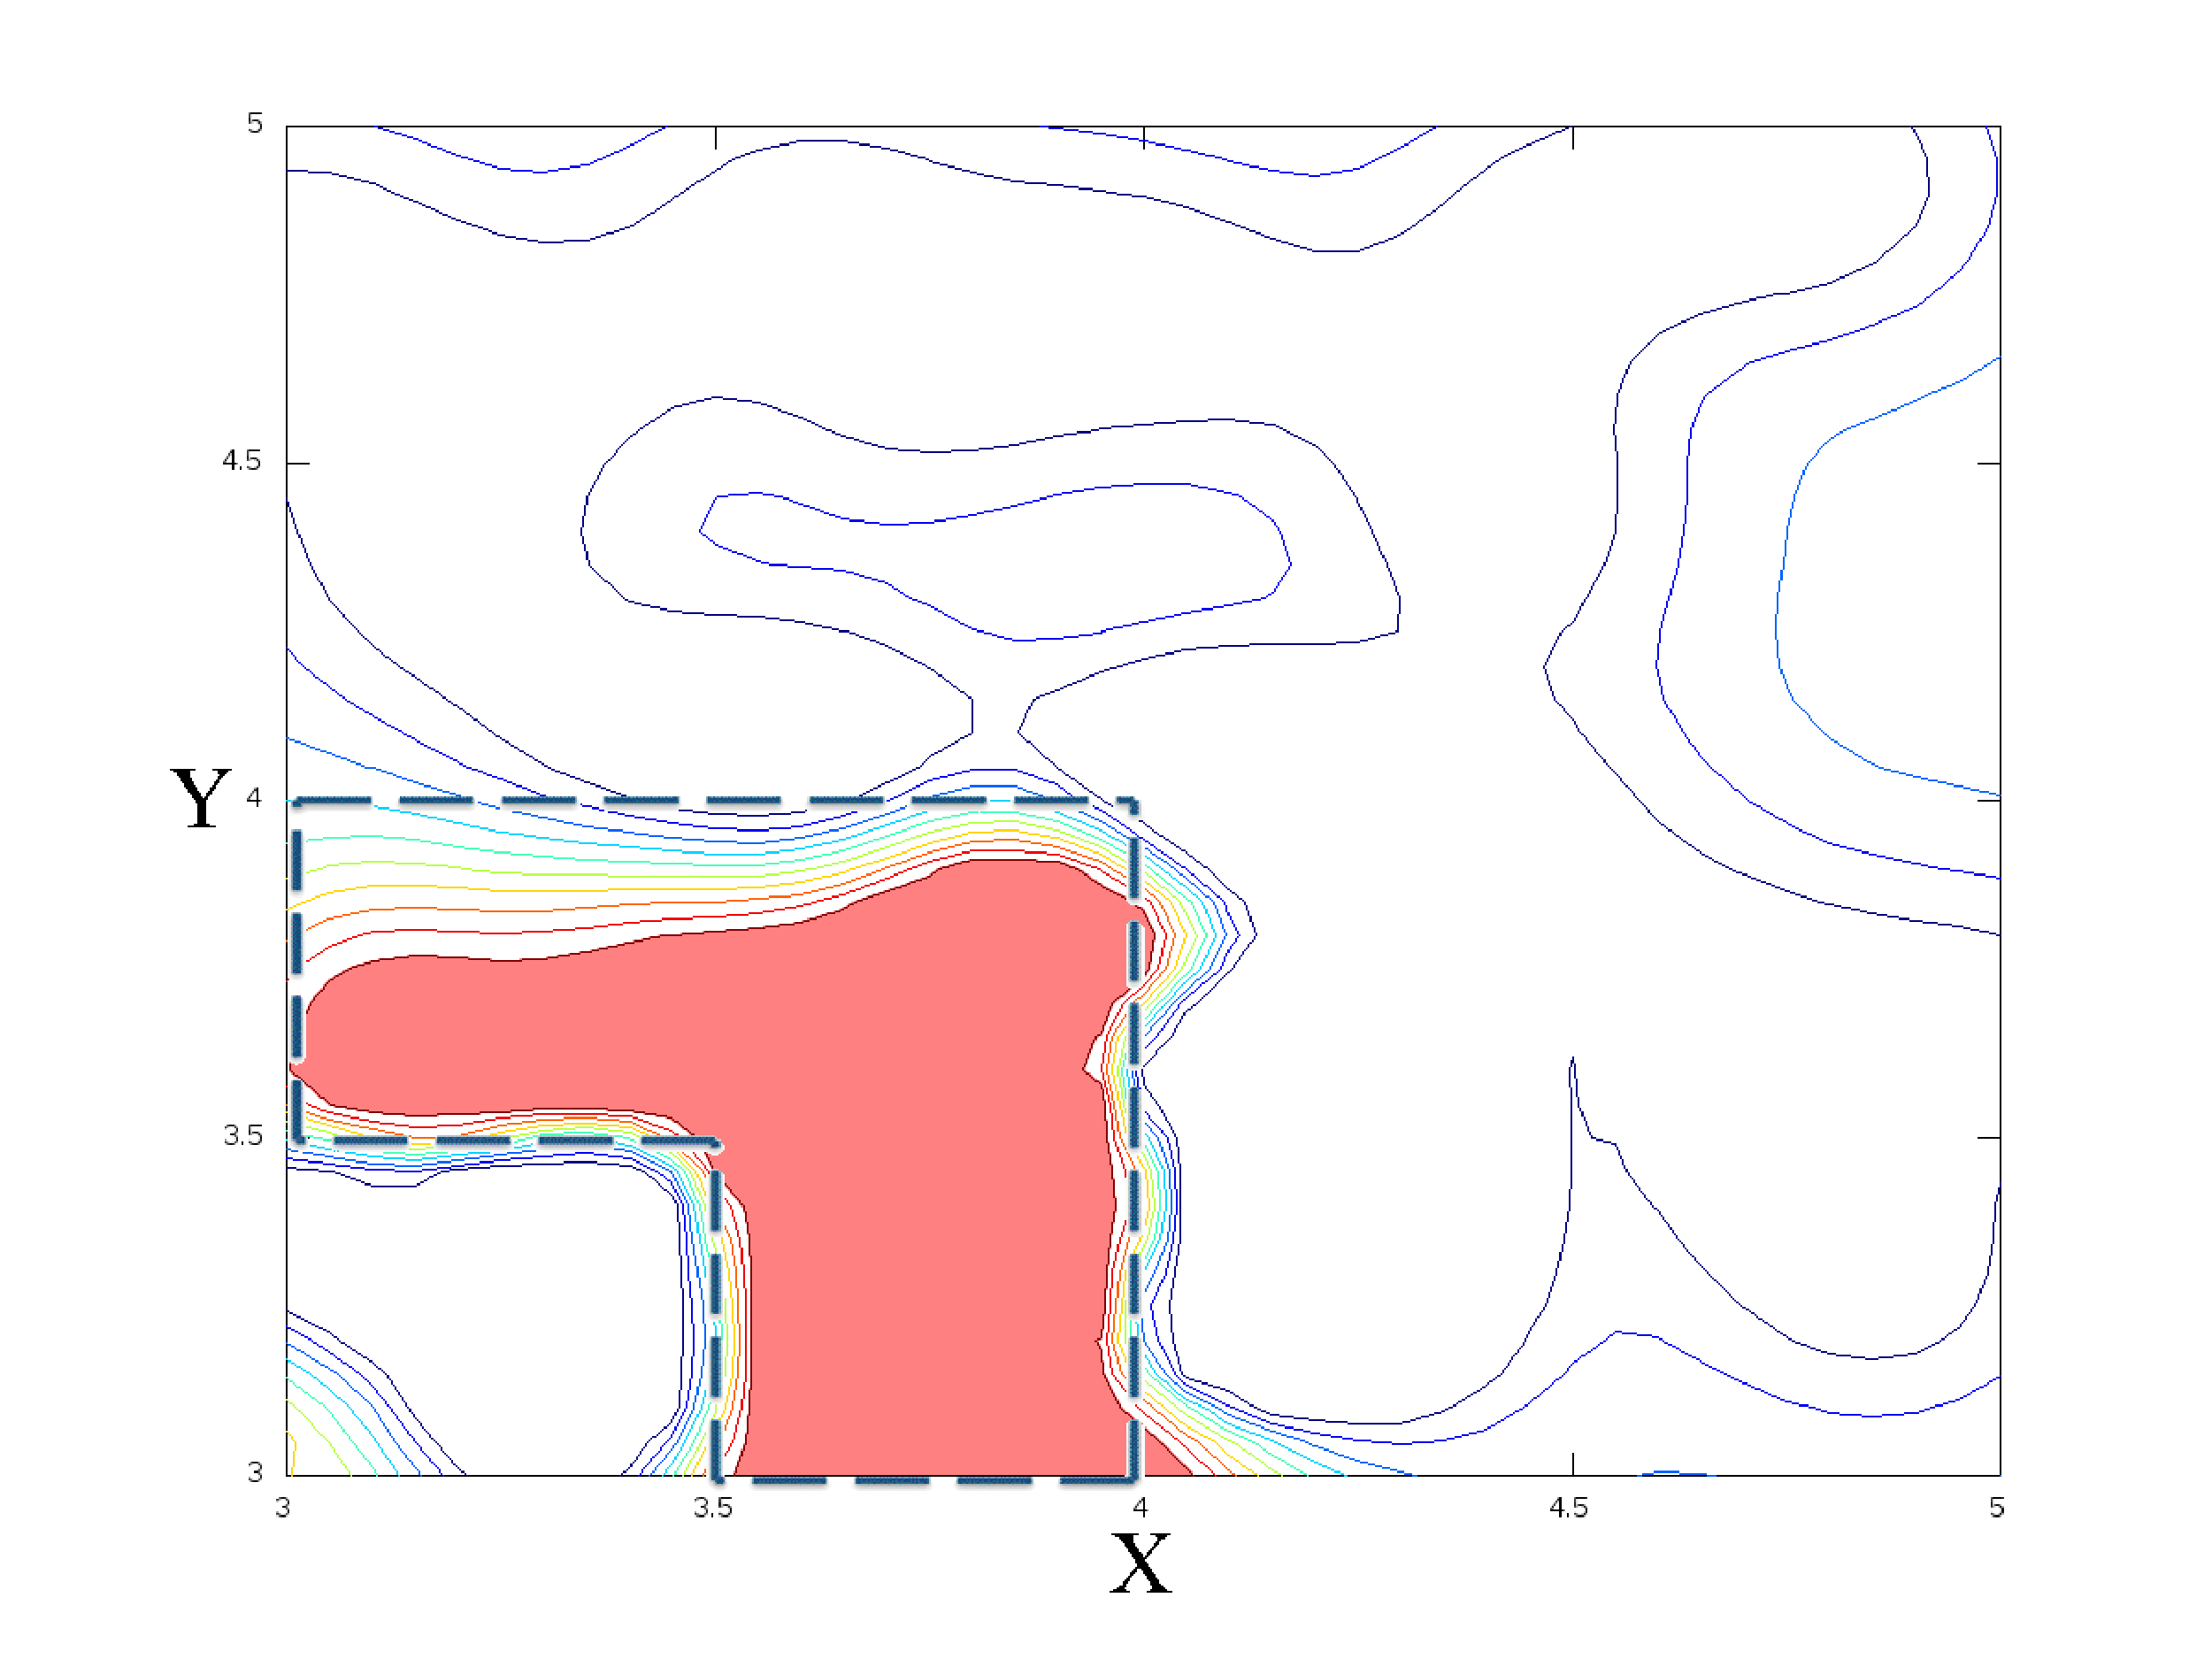
\includegraphics[width=0.75\linewidth]{images/toy2svm}
  \caption{
    Contour of the trained SVMs for the second toy problem (Table \ref{tab:parkour_cmac}).
    The feasible region classified by SVMs is filled with red. The
    ground truth feasible region is outlined by the dashed lines.
    For clarity, the figure is zoomed into the region from $[-5,5]^2$ to $[3, 5]^2$ .
  }
  \label{fig:parkour_cmac}
\end{figure}

We compared the performance of standard CMA-ES and CMA-C on each
problem by evaluating 20 times with different initial seeds.
%% \original{
%% On average, CMA-C is four to five times faster than standard CMA-ES (Table
%% \ref{tab:cmac}). 
%% }
%% \updated{
%% On average, CMA-C evaluates four to five times less than standard CMA-ES
%% (Table \ref{tab:cmac}). 
%% In our toy examples, the number of evaluations is more critical than the timing
%% because calculating the cost function is a bottle neck of real problems
%% and additional training time of classifiers becomes negligible.
%% }
For a problem with costly sample
evaluation routines, such as the controller design problem focused in
this paper, CMA-C significantly reduces the total computation
time. However, if the sample evaluation time is negligible, such as
our toy examples, reducing the number of evaluations does not speed
up the total computation time. In fact, CMA-C can be slower than
CMA-ES due to the additional computation on constructing SVMs.

To further evaluate the performance of CMA-C, we conducted two sets of
analyses by varying the ratio of the infeasible area to the feasible
area (problem I) and the level of noise (problem II).  Both analyses
were designed to add difficulty in finding feasible solutions to the
optimization problem. Our results, shown in Table
\ref{tab:parkour_toy_area_ratio_test} and Table \ref{tab:parkour_toy_noise_test},
indicate that the performance of CMA-C increases when either the
magnitude of the noise in the infeasible region or the infeasible area increases,
while the frequency of noise does not have
a significant correlation to the performance gain.
%% \revthree{while the frequency of noise does not affect the performance gain.}

In addition, we validated the approximated feasible regions by
visualizing the difference between constructed SVM and the ground
truth (\figref{parkour_cmac}). The results show that the non-convex SVM boundary in
the second problems match the ground truth well. The only difference resides
in the upper left corner of the L-shape feasible region in the second
problem. 
%% This result is reasonable because the optimal solution lies
%% in the upper corner, which biases CMA to sample less frequently in the
%% lower corner.


\subsection{Analysis on Real Problems}
We also evaluated the performance of CMA-C on the problems of
controller design (Table \ref{tab:parkour_cmac}). On average, CMA-C performed
five times faster than CMA-ES to achieve the same optimal value. In
some cases, CMA-C reached desired objective value, while CMA-ES got
stuck in the local minima. The advantage of CMA-C is even more
prominent when solving a series of optimizations with gradually
introduced constraints, because CMA-C can simply overlap the new SVM
with previously constructed ones. However, when the infeasible region
is relatively small, the difference in performance between CMA-C and
CMA-ES is not obvious. For example, thrusting controller does not
fully exploit the advantages of CMA-C due to its relatively small
infeasible region.


